\documentclass[20pt]{article}
\usepackage[T2A]{fontenc}
\usepackage{mathtools}
\usepackage[utf8]{inputenc}
\usepackage[english, russian]{babel}
\usepackage{fancyhdr}
\usepackage{graphicx}
\usepackage{gensymb}
\usepackage{floatrow}

\pagestyle{fancy}
\author{}
\title{Определение $C_p/C_v$ по скорости звука в газе}
\lhead{Работа 2.1.3 (5)}
\rhead{Терехов Максим 876}
\date{}

\begin{document}
\selectlanguage{russian}
\parindent=1cm
\large
\maketitle
\section{Цель работы:}
1) измерение частоты колебаний и длины волны при резонансе звуковых колебаний в газе, заполняющем трубу;
2) определение показателя адиабаты с помощью уравнения состояния идеального газа.
\section{В работе используются:}
звуковой генератор, электронный осциллограф, теплоизолированная труба, обогреваемая водой из термостата, термостат, телефон, соединённый с генератором звука, микрофон, соединённый с осциллографом.
\section{Экспериментальная установка:}
\begin{figure}[H]
\center
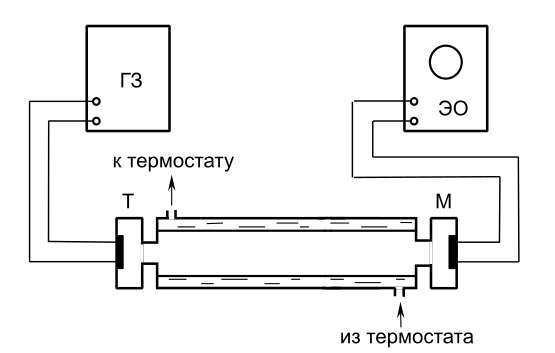
\includegraphics[scale=0.5]{asd.png}
\end{figure}
\section{Теоретическая часть:}	

Скорость распространения звуковой волны в газах зависит от показателя адиабаты $\gamma$. На измерении скорости звука основан один из наиболее точных методов определения показателя адиабаты.

Скорость звука в газах определяется формулой:
\[
	c = \sqrt{\gamma \frac{RT}{\mu}},
\]
где $R$ --- газовая постоянная, $T$ --- температура газа, а $\mu$ --- его молярная масса. Преобразуя эту формулу, найдем
\begin{equation}
	\gamma = \frac{\mu}{RT} c^2.
\end{equation}
Таким образом, для определения показателя адиабаты достаточно измерить температуру газа и скорость распространения звука (молярная масса газа предполагается известной).

Звуковая волна, распространяющаяся вдоль трубы, испытывает
многократные отражения от торцов. Звуковые колебания в трубе являются наложением всех отраженных волн и, вообще говоря, очень сложны. Картина упрощается, если длина трубы $L$ равна целому числу полуволн, то есть когда
\begin{equation}
	L = n \lambda/2,
\end{equation}
где $\lambda$ --- длина волны звука в трубе, а $n$ --- любое целое число. Если условие (2) выполнено, то волна, отраженная от торца трубы, вернувшаяся к ее началу и вновь отраженная, совпадает по фазе с падающей. Совпадающие по фазе волны усиливают друг друга. Амплитуда звуковых колебаний при этом резко возрастает --- наступает
резонанс.
При звуковых колебаниях слои газа, прилегающие к торцам трубы, не испытывают смещения (\itshape узел смещения\rm ). Узлы смещения повторяются по всей длине трубы через $\lambda/2$. Между узлами находятся
максимумы смещения (\itshape пучности\rm ).

Скорость звука c связана с его частотой $f$ и длиной волны $\lambda$ соотношением
\begin{equation}
	c = \lambda f.
\end{equation}
Для получения резонанса при постоянной длине трубы можно изменять частоту звуковых колебаний. В этом случае следует плавно изменять частоту $f$
звукового генератора, а следовательно, и длину звуковой волны $\lambda$.
Для последовательных резонансов получим
\begin{equation}
L_n = \frac{\lambda_1}{2}n=\frac{\lambda_2}{2}(n+1) = \ldots = \frac{\lambda_{k+1}}{2}(n+k)
\end{equation}
Из (3) и (4) имеем
\[
	f_1 = \frac{c}{\lambda_1} = \frac{c}{2L}n, \quad f_2 = \frac{c}{\lambda_2} = \frac{c}{2L}(n+1) = f_1 + \frac{c}{2L},\quad \ldots,
\]
\begin{equation}
f_{k+1} = \frac{c}{\lambda_{k+1}} = \frac{c}{2L}(n+k)= f_1 + \frac{c}{2L}k.
\end{equation}
Скорость звука, деленная на $2L$, определяется, таким образом,
по угловому коэффициенту графика зависимости частоты от номера
резонанса.
\section{Обработка результатов измерений:}
Исследуемый газ --- воздух.
\[
	P = 974.2 \cdot 10^2\ \text{Па} \qquad L = 70\ \text{см}
\]
\\
\begin{center}
\begin{tabular}{|c|c|c|c|c|}
\hline
$T_1, K$ & $T_2, K$ & $T_3, K$ & $T_4, K$ & $T_5, K$ \\\hline
$297$ & $303$ & $313$ & $323$ & $333$ \\\hline
\end{tabular}
\end{center}
\begin{center}
\begin{tabular}{|c|c|c|c|c|c|c|}
\hline
$T_1$ & $f_1,\ \text{Гц}$ &$f_2,\ \text{Гц}$ &$f_3,\ \text{Гц}$ &$f_4,\ \text{Гц}$ &$f_5,\ \text{Гц}$ & $f_6,\ \text{Гц}$\\\hline
 $$ & $247$ & $498$ & $720$ & $980$ & $1220$ & $1458$ \\\hline
\end{tabular}
\end{center}
\begin{center}
\begin{tabular}{|c|c|c|c|c|c|c|}
\hline
$T_2$ & $f_1,\ \text{Гц}$ &$f_2,\ \text{Гц}$ &$f_3,\ \text{Гц}$ &$f_4,\ \text{Гц}$ &$f_5,\ \text{Гц}$ & $f_6,\ \text{Гц}$\\\hline
 $$ & $257$ & $502$ & $749$ & $992$ & $1221$ & $1476$ \\\hline
\end{tabular}
\end{center}
\begin{center}
\begin{tabular}{|c|c|c|c|c|c|c|}
\hline
$T_3$ & $f_1,\ \text{Гц}$ &$f_2,\ \text{Гц}$ &$f_3,\ \text{Гц}$ &$f_4,\ \text{Гц}$ &$f_5,\ \text{Гц}$ & $f_6,\ \text{Гц}$\\\hline
 $$ & $260$ & $511$ & $760$ & $1014$ & $1265$ & $1512$ \\\hline
\end{tabular}
\end{center}
\begin{center}
\begin{tabular}{|c|c|c|c|c|c|c|}
\hline
$T_4$ & $f_1,\ \text{Гц}$ &$f_2,\ \text{Гц}$ &$f_3,\ \text{Гц}$ &$f_4,\ \text{Гц}$ &$f_5,\ \text{Гц}$ & $f_6,\ \text{Гц}$\\\hline
 $$ & $264$ & $519$ & $771$ & $1035$ & $1272$ & $1536$ \\\hline
\end{tabular}
\end{center}
\begin{center}
\begin{tabular}{|c|c|c|c|c|c|c|}
\hline
$T_5$ & $f_1,\ \text{Гц}$ &$f_2,\ \text{Гц}$ &$f_3,\ \text{Гц}$ &$f_4,\ \text{Гц}$ &$f_5,\ \text{Гц}$ & $f_6,\ \text{Гц}$\\\hline
 $$ & $270$ & $524$ & $780$ & $1045$ & $1311$ & $1565$ \\\hline
\end{tabular}
\end{center}
Построим графики, откладывая по оси абсцисс номер резонанса $k$, а по оси ординат --- разность между частотой последующих резонансов и частотой первого резонанса:
$f_{k+1}-f_1$. Угловой коэффициент прямой определяет величину $c/2L$.
 \begin{figure}[H]
	\caption{График зависимости разности частот от номера резонанса при $T_1$}
	\center
	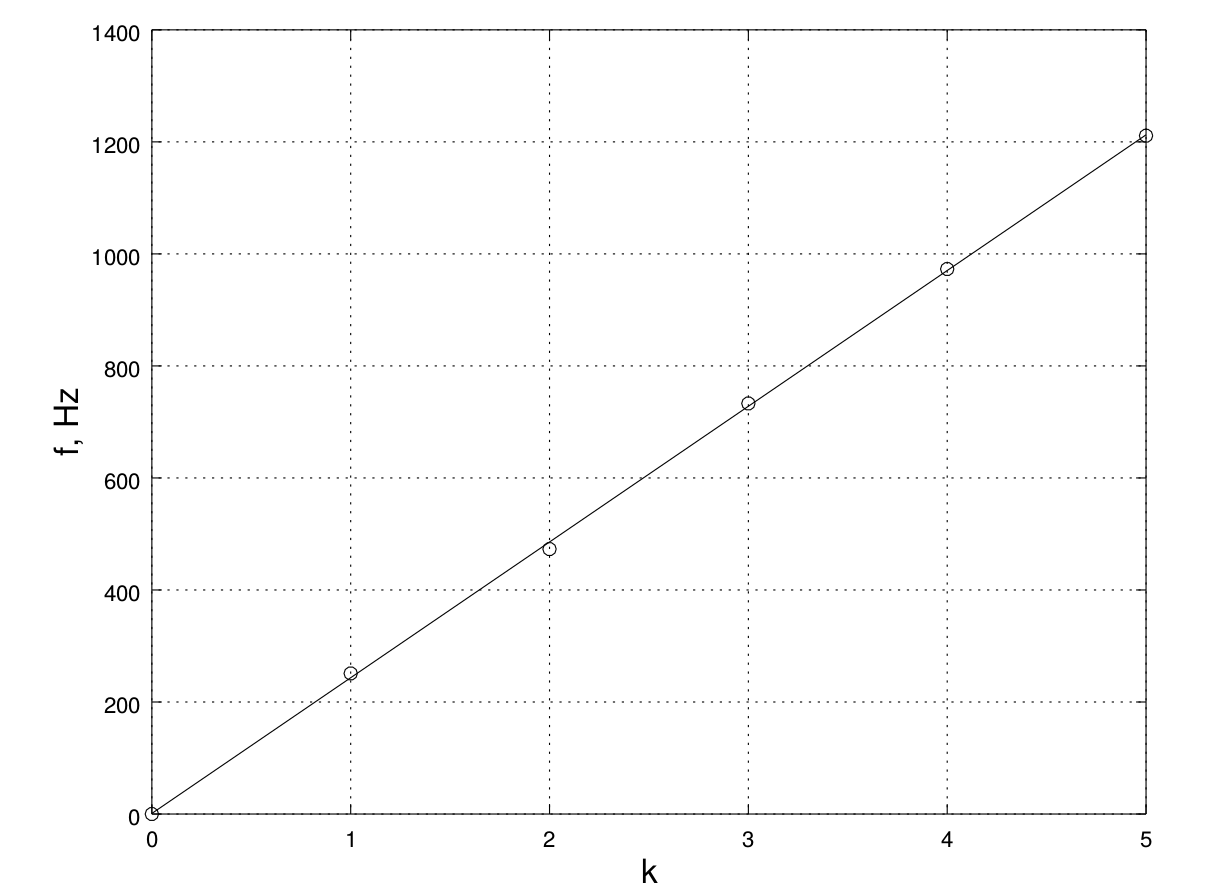
\includegraphics[scale=0.25]{T1.png}
\end{figure}
 \begin{figure}[H]
	\caption{График зависимости разности частот от номера резонанса при $T_2$}
	\center
	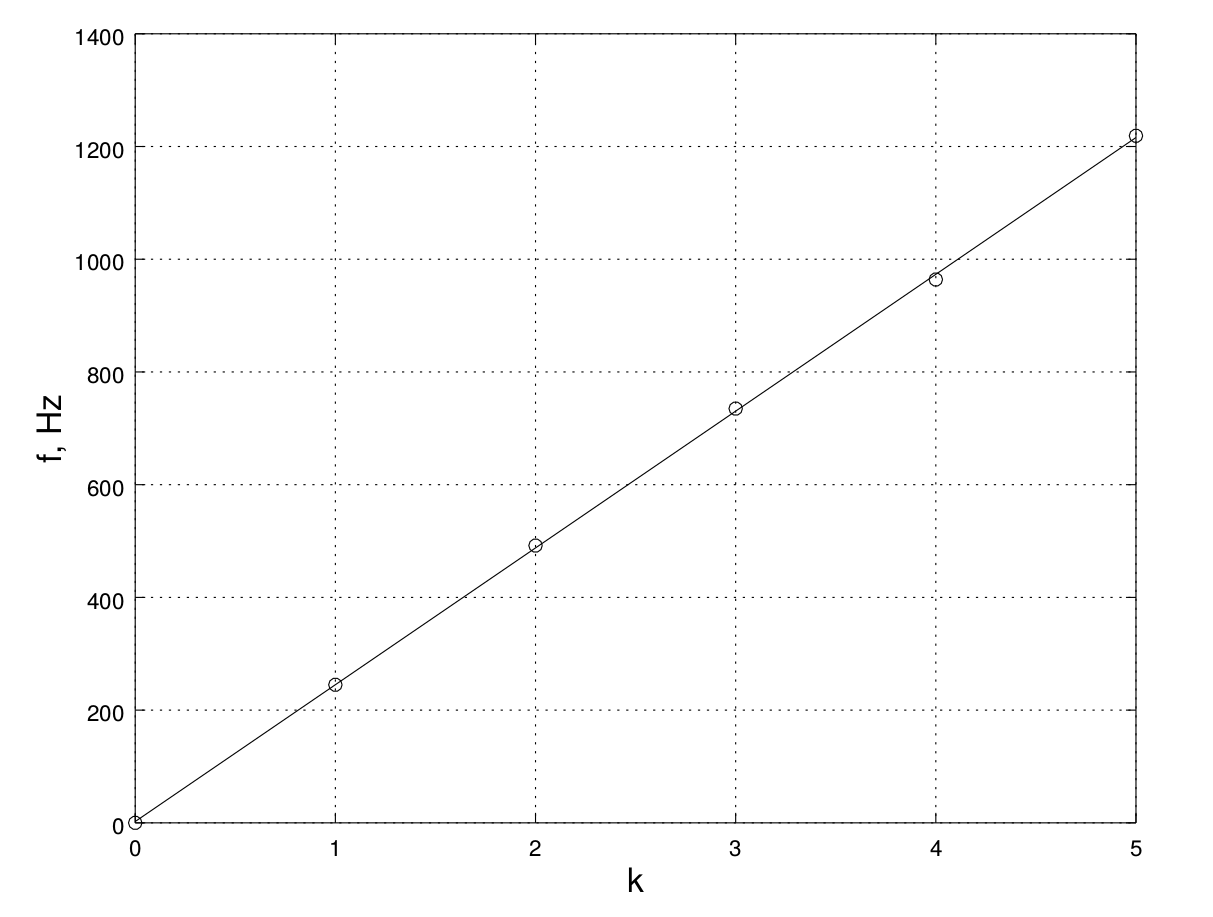
\includegraphics[scale=0.25]{T2.png}
\end{figure}
 \begin{figure}[H]
	\caption{График зависимости разности частот от номера резонанса при $T_3$}
	\center
	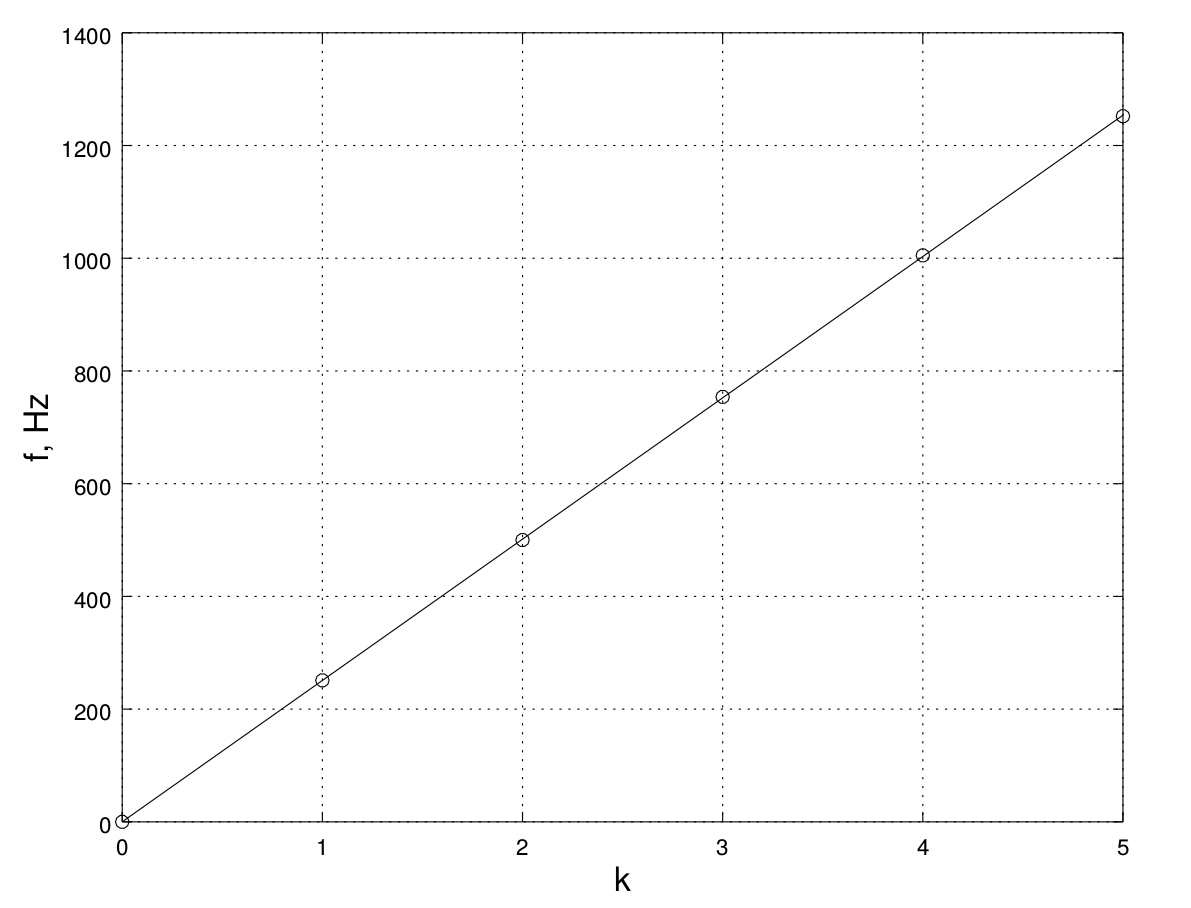
\includegraphics[scale=0.25]{T3.png}
\end{figure}
 \begin{figure}[H]
	\caption{График зависимости разности частот от номера резонанса при $T_4$}
	\center
	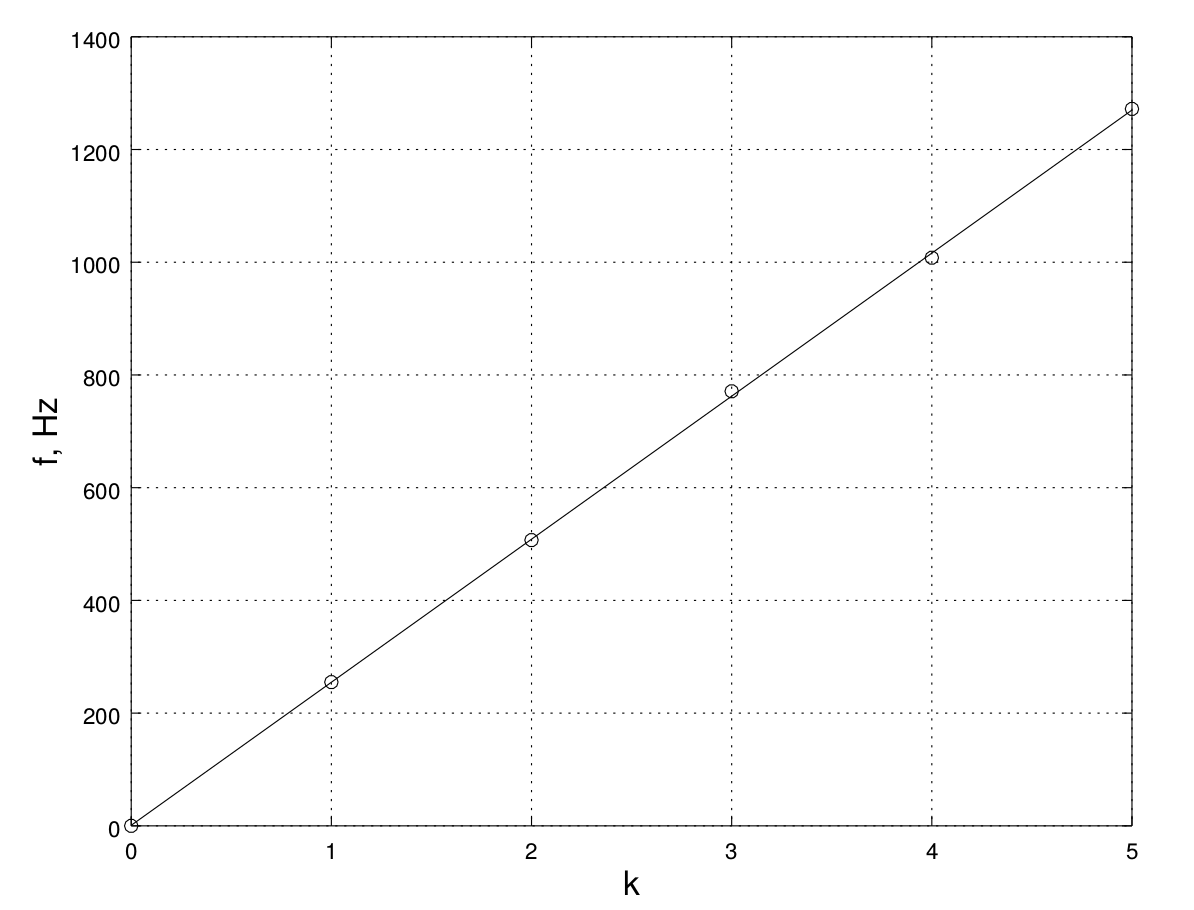
\includegraphics[scale=0.25]{T4.png}
\end{figure}

 \begin{figure}[H]
	\caption{График зависимости разности частот от номера резонанса при $T_5$}
	\center
	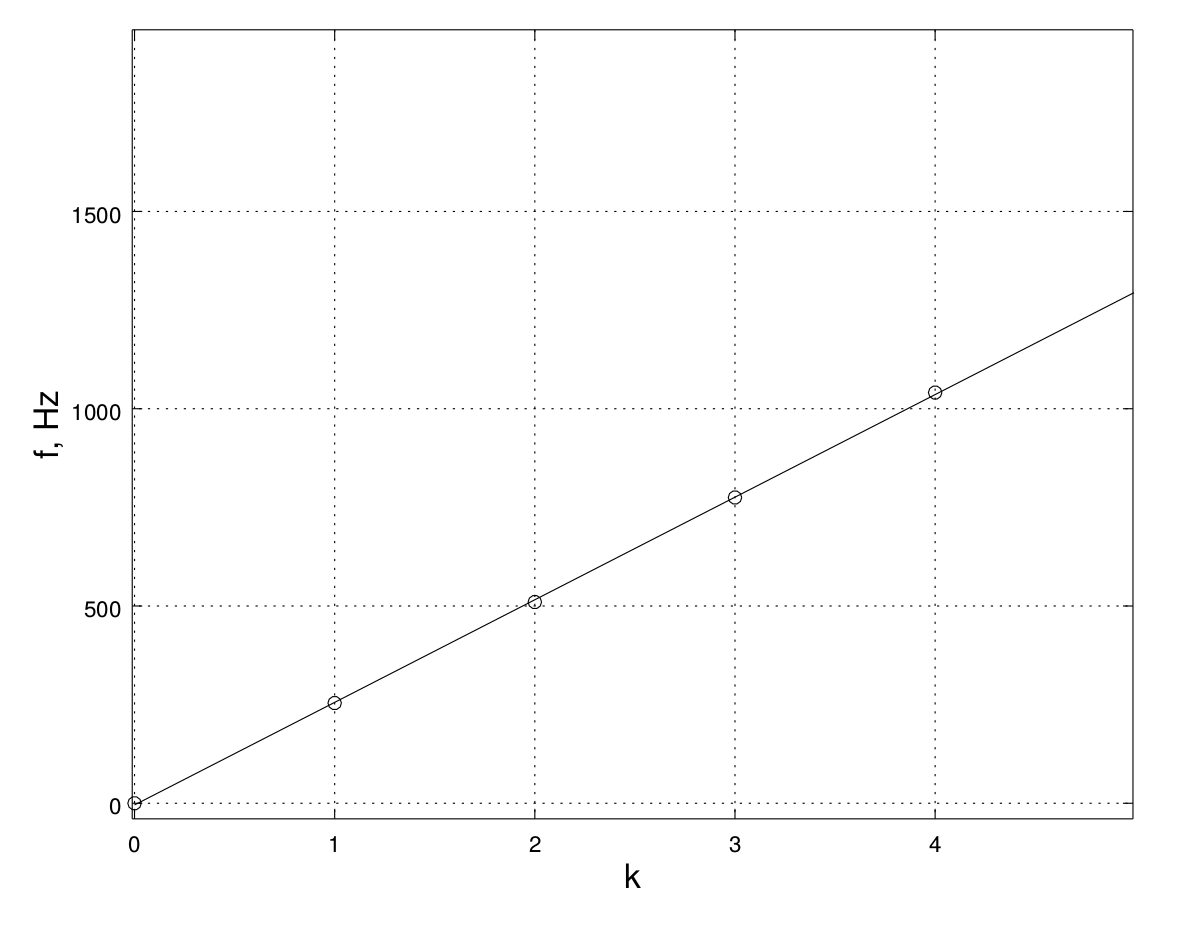
\includegraphics[scale=0.25]{T5.png}
\end{figure}

Угловые коэффициенты прямых соответственно равны:
\[
	a_1 = 246.59\ c^{-1}, \quad a_2 = 249.81\ c^{-1}, \quad a_3 = 252.99\ c^{-1}, 
\]
\[	
	\quad a_4 = 256.91\ c^{-1}, \quad a_5 = 260.85\ c^{-1}.
\]
Рассчитаем скорость звука и показатель адиабаты при каждой температуре по формулам (1) и (5):
\\
\begin{center}
\begin{tabular}{|c|c|c|}
\hline $T,\ K$ & $c,\ \text{м/с}$ & $\gamma$ \\\hline
$297$ & $345.22$ & $1.400$ \\\hline
$303$ & $349.74$ & $1.402$ \\\hline
$313$ & $354.18$ & $1.399$ \\\hline
$323$ & $359.67$ & $1.398$ \\\hline
$333$ & $365.19$ & $1.398$ \\\hline
\end{tabular}
\end{center}
Оценим погрешности:
\[
\varepsilon_{T} = 0.003 = 0.3\%
\]
\[
\varepsilon_{f} = 0.009 = 0.9\%
\]
\[
 \varepsilon_c = \sqrt{\varepsilon_{T}^2 + \varepsilon_{f}^2} = 0.0124 = 1.24\%
\]
\[
	\varepsilon_{\gamma} = 2 \varepsilon_c + \varepsilon_T = 0.0318 = 3.18\%
\]
Конечный ответ:
\[
	\gamma = 1.399 \pm 0.05
\]
Табличное значение:
\[
	\gamma_{\text{табл}} = 1.403
\]
\end{document}
